\chapter{結論與未來展望}
\section{結論}\label{s5.1}
\indent
本論文基於呂昭陞論文提出XPath撰寫樣式的使用前提下,
為減少在挑選適合的路徑條件所花用的時間,而提出利用HTML比對的瀏覽器擴充元件找出適合的元件定位條件。

使用者一般在查找變化時,通常都會使用瀏覽器中的Developer Tools來觀察元件是否有淺紫背景框,
但這個方法較慢又容易忽略一些更適合當成XPath路徑條件的變化。
此擴充元件透過HTML比對,將有變化的元件列舉出來,讓使用者可以直接透過結果挑選適合的變化加入XPath的路徑條件中。
從實驗結果可以得知,
無論是無相關經驗或已經有一定基礎的測試人員使用Developer Tools配合此擴充元件查找變化,
和僅使用Developer Tools的情況相比,時間減少$20\%\sim30\%$左右,
尤其無相關經驗的測試人員減少的時間會更多一些。
由此可知,透過Developer Tools加上擴充元件的輔助可以降低設計XPath所花用時間,提高撰寫測試腳本的效率。

\section{未來方向}\label{s5.2}
\indent
本論文提出之HTML比對工具仍有待改善之處,以下將分為五點說明:

\subsection{比較節點相異等級之演算法}\label{s5.2.1}

本論文使用的HTML比對程式,
計算節點相異的等級有分成``IDENTICAL''、``SAME BUT DIFFERENT''和``NOT THE SAME NODE''三種類型。
判斷節點相異的演算法是先設定每個屬性的權重,並將該節點所擁有的屬性權重全部相加,最後計算後的結果來決定該節點的相異等級。

使用這種演算法的時候,在判定``SAME BUT DIFFERENT''和``NOT THE SAME NODE''這兩種類型時,
沒辦法精確的判定相異等級,
像是圖\ref{f5.1}中以使用者的角度會知道它是id=``456''的節點刪除,
但以原本的演算法會因為節點等級,
而判斷成id=``456''的元件修改成id=``789''的元件,原本id=``789''的元件則會被刪除。
若能調整判斷節點的演算法,使它更能趨近使用者的結果,最後輸出的節點變化類型也會更精確。

\indent
\begin{figure}[H]
    \centering
    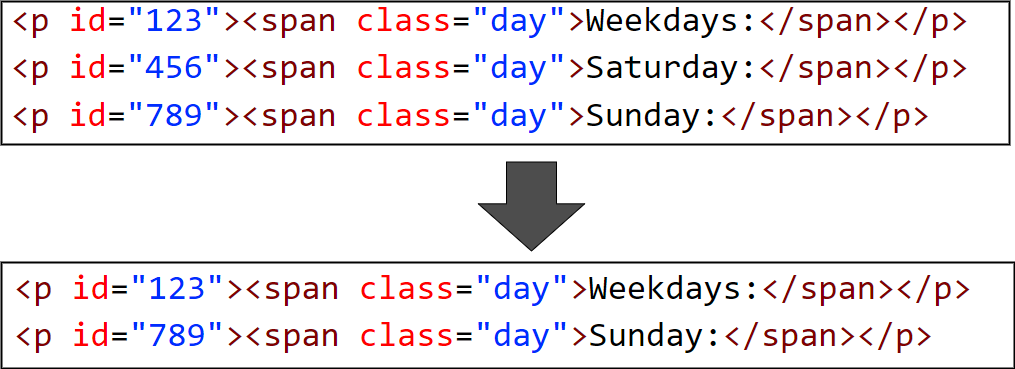
\includegraphics[width=0.8\textwidth]{picture/ch-5 Heuristic_improve.png}
    \caption{比較節點相異等級之情境}
    \label{f5.1}
\end{figure}

\subsection{比對相異之元件自動跳轉到Develope Tool中Element頁面並標記}\label{s5.2.2}

此工具在顯示結果時,僅告訴使用者變化元件的路徑,
使用者必須照著路徑一個一個慢慢找出元件在該HTML的位置,
或透過畫面上的元件變化直接用Developer Tools中``Inspect Element''功能找出元件後,再利用路徑查看是不是比較結果中的元件,
若以上述的兩種作法操作,使用速度及方便度會降低。
若查看比較結果時,
可以讓使用者直接跳轉到Developer Tools中Element頁面上的該元件,
會讓使用者可以快速的觀察出變化並設計XPath表達式。

\subsection{比對結果過濾功能新增}\label{s5.2.3}

目前此工具建立了三個可以過濾結果的選項,
可以依照使用者的當下的情況來過濾掉不需要的結果,
讓使用者能更快速地找出XPath表達式中的路徑條件,
若增加更多過濾的情境,
便可以在查找變化前先把大部分的無用結果先篩選掉。

\subsection{紀錄多個狀態的HTML}\label{s5.2.4}

目前的設計僅能儲存開始計時前和計時後的兩個HTML;
若能增加暫存功能,
能記錄多個狀態的HTML並且挑選其中兩個狀態的HTML來進行比對,
也會加快使用者操作的方便性,
不用等待計時器和程式的運行時間,

\subsection{UI/UX介面美化及操作更人性化}\label{s5.2.5}

在設計UI介面時,僅用基本的顏色和元件來進行簡單的操作;
而UX介面是以較大的字樣以及元件為主軸,會造成頁面上會常常使用到滾輪來移動顯示畫面。
若在視窗中加上分頁或下拉選單等等可以隱藏部分元件的設計,
可以使得頁面更加簡潔,讓使用者在操作時也會更順手。